\chapter{总体设计}

\section{系统设计}

\begin{figure}[H]  % "h!" 表示尽可能在当前位置插入
    \centering  % 图片居中
    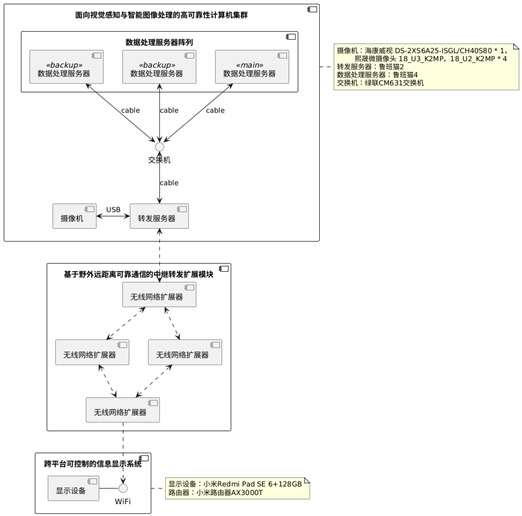
\includegraphics[width=1.0\textwidth]{architecture.png}  % 图片文件路径,设置宽度为页面宽度的80%
    \caption{系统架构图}  % 图片标题
    \label{fig:architecture}
\end{figure}

本项目总体上分为图像处理系统、数据传输系统、信息显示系统三个部分。

图像处理系统由摄像头、转发服务器和处理服务器阵列构成。摄像头负责图像数据的采集,并支持一定程度的变焦功能,能够根据接收的指令自动变焦。摄像头通过USB数据线有线连接到转发服务器。转发服务器负责监控处理服务器阵列的运行状况,并将待处理的图像转发给处理服务器阵列。处理服务器阵列则负责对接收到的图像进行深度学习检测,以识别危险情况。如果发现存在危险,则控制摄像头进行变焦,拍摄更为清晰的危险画面;如已达到摄像头变焦极限,则自动对危险区域进行裁剪。转发服务器与所有处理服务器通过有线连接构成计算机网络,使用星形拓扑,可以直接使用集线器进行组网,转发服务器为中心。只要至少还有一个处理服务器正常运行,就不影响系统的正常运行。转发服务器和处理服务器使用TCP协议进行连接。处理服务器阵列为一主多备架构,当前正在负责图像处理任务的服务器为主服务器,其余为备用服务器。所有处理服务器均需定时与转发服务器通信,以告知转发服务器每个处理服务器的存活状态。当主处理服务器崩溃时,转发服务器发现通信连接丢失,自动启用一个备用服务器作为主服务器。崩溃的主服务器应当自行尝试重启并尝试与转发服务器建立连接.

数据传输系统为图像处理系统与信息显示系统之间的桥梁。该模块由多个WiFi中继器构成,通过利用WiFi中继器扩大无线网络范围。WiFi中继器应当构成环形拓扑,以增强网络可靠性:当任何一个中继器崩溃时,仍不影响系统正常运行。显示模块是面向用户的外部子系统,该模块包括一块显示屏。显示屏自带创建WiFi的功能,系统中所有的设备均直接或间接地连接到显示屏创建的WiFi中。

信息显示系统为若干支持浏览器功能与无线网络功能的终端设备。用于显示系统处理后的图像和其他信息。

\section{处理流程}

转发服务器通过连接的摄像头获取图像,并发送到当前启用的图像处理服务器进行危险情况识别。然后将识别结果通过无线网络发送到终端设备进行显示。同时接收终端设备的控制请求如缩放、变焦等操作,并进行对应的处理。